\subsection{Uso de MLOps mediante despliegue en un ambiente controlado, con la capacidad de monitorear y mejorar continuamente el rendimiento del modelo}

\subsubsection{Despliegue en Cloud}

La plataforma DAGsHub se presenta como una solución integral específicamente diseñada para la ingeniería de software, fusionando de manera efectiva las funcionalidades esenciales de control de versiones del código, versionado de datos y seguimiento de experimentos. Este enfoque unificado facilita la administración de proyectos en los campos de aprendizaje automático, desde la fase inicial de experimentación hasta la colaboración en equipo y la entrega de resultados. \newline

La integración de DAGsHub con herramientas clave como Git, DVC y MLFlow fortalece aún más su versatilidad. Cada una de estas herramientas desempeña un papel específico y complementario en el proceso. Git se encarga del control de versiones del código, DVC se especializa en la gestión de datos, mientras que MLFlow se enfoca en el seguimiento de experimentos y versionado de modelos. Esta plataforma permite a cada herramienta cumplir eficientemente su función designada, optimizando así el flujo de trabajo en cada aspecto del proyecto.

\newpage

\begin{figure}[h]
\centering
\caption{Plataforma que integra el versionado del código, los datos y los modelos – DagsHub}
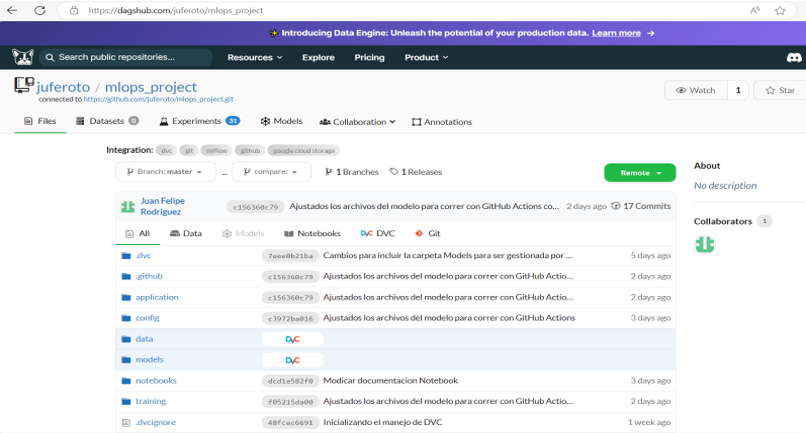
\includegraphics[width=1\textwidth]{resultados/herramientaDagshub.png}
\caption*{\footnotesize Fuente: Elaboración propia}
\label{fig:figuraHerramientaDagshub}
\end{figure}

Al acceder a la interfaz de DAGsHub mediante el enlace detallado\footnote{El código de DagsHub se encuentra \href{https://dagshub.com/juferoto/mlops_project}{aquí}.}, se inicia el proceso para utilizar esta plataforma. Para dar inicio a su uso, es posible crear una cuenta de forma gratuita. Esta suscripción no conlleva ningún costo y permite gestionar proyectos públicos sin restricciones. El límite máximo para el espacio de almacenamiento es de 100 gigabytes, proporcionando así un entorno accesible y eficiente para el manejo de datos en proyectos específicos. \newline

La configuración del proyecto sigue la misma estructura que se detalló en el objetivo 3, tal como se describe en la figura \ref{fig:figuraHerramientaDagshub}. Al crear una cuenta en DAGsHub, esta se vincula automáticamente con la cuenta Github utilizada para el versionado del código. Posteriormente, al compartir el enlace, se posibilita a otros usuarios acceder a la configuración del proyecto de manera sencilla. Este enfoque facilita la colaboración y el intercambio de información entre los miembros del equipo alineando la integración del proyecto de manera eficiente. \newline

Cuando se busca incorporar almacenamiento externo, se presentan dos opciones específicas: AWS (Amazon S3) y Google Cloud (Google Storage). En este proyecto en particular, se optó por utilizar Google Cloud Storage (ver figura \ref{fig:figuraOpcionesAlmacena}). Al hacer clic en la opción correspondiente, se despliegan las configuraciones necesarias, permitiendo así realizar las acciones pertinentes para integrar y agregar el almacenamiento en la nube de Google al proyecto. Este proceso se simplifica mediante una interfaz intuitiva que guía al usuario a través de las opciones necesarias para una configuración eficaz.

\begin{figure}[h]
\centering
\caption{Opciones para configurar un almacén de datos en DagsHub}
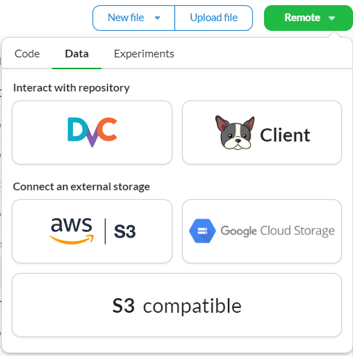
\includegraphics[width=0.7\textwidth]{resultados/opcionesAlmacena.png}
\caption*{\footnotesize Fuente: Elaboración propia}
\label{fig:figuraOpcionesAlmacena}
\end{figure}

\newpage

Al seleccionar la opción ``Remote’’, se habilita la capacidad de visualizar los experimentos realizados con MLFlow (ver figura \ref{fig:figuraOpcionesMLFlow}). Es importante destacar que, en este contexto, la visualización no ocurre a nivel local, sino que se realiza de forma remota a través de la plataforma proporcionada por DagsHub con la “Go to mlflow UI”. Esto implica que los datos y resultados almacenados en MLFlow se encuentran accesibles de manera remota, gracias a la integración facilitada por DagsHub.


\begin{figure}[h]
\centering
\caption{Opciones para usar remotamente MLFlow}
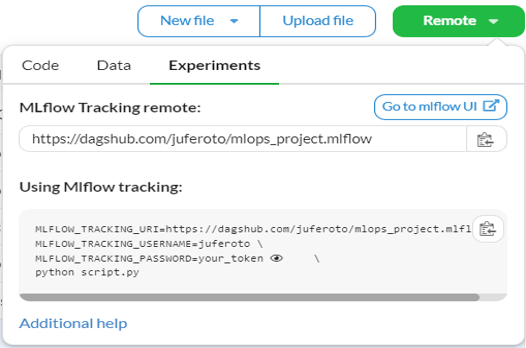
\includegraphics[width=0.8\textwidth]{resultados/opcionesMLFlow.png}
\caption*{\footnotesize Fuente: Elaboración propia}
\label{fig:figuraOpcionesMLFlow}
\end{figure}

Para contextualizar y entender cómo se integra MLFlow en la nube con DagsHub, es esencial considerar los ajustes necesarios en el archivo principal ``main.yml’’ de configuraciones. Al hacer la comparación, se identifica que en la configuración de MLFlow para trabajar en la nube, se requiere la adición de la URL que indica la ubicación específica del proyecto proporcionado por DagsHub, como el usuario y contraseña que provee DagsHub. Estos ajustes permiten que el proyecto se conecte con los recursos en la nube de MLFlow, facilitando así la gestión y visualización remota de experimentos y datos asociados con el proyecto realizado.

\newpage

\begin{figure}[h]
\centering
\caption{Configuración remota del MLFlow en el archivo ``main.yml''}
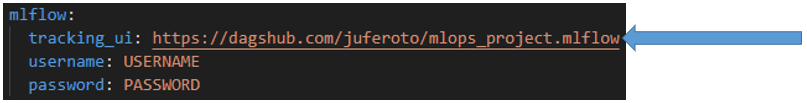
\includegraphics[width=1\textwidth]{resultados/confRemotaMLFlow.png}
\caption*{\footnotesize Fuente: Elaboración propia}
\label{fig:figuraOpcionesMLFlow}
\end{figure}

El enlace específico del proyecto que provee DagsHub para MLflow es \href{https://dagshub.com/juferoto/mlops_project.mlflow}{https://dagshub.com/juferoto/mlops_project.mlflow}. Este enlace es el que se debe sustituir en el archivo correspondiente\footnote{Dentro del video se demuestra la gestión remota de la herramienta MLflow, siguiendo un proceso similar al realizado localmente. La diferencia clave radica en que esta vez se realiza de manera remota. El enlace para acceder al video se encuentra disponible para su visualización en YouTube \href{https://youtu.be/U2DqNOixHWw?si=OrJcIFpGiqfodAQy}{aquí}.}, tal como se señala en la imagen anterior.

Siguiendo con el despliegue en la nube, con el objetivo de asegurar un funcionamiento sin contratiempos tanto para la aplicación como para la API, es crucial determinar las dependencias necesarias. Por esta razón, se genera un archivo llamado requirements.txt., Este archivo se crea para enumerar todas las dependencias esenciales. La instalación de estas dependencias se lleva a cabo mediante el comando 
\begin{verbatim}
pip install -r requirements.txt
\end{verbatim} 

Este proceso garantiza que todas las herramientas y dependencias necesarias se instalen de manera coherente, proporcionando así las condiciones apropiadas para el correcto funcionamiento de la aplicación y la API en la nube.


\newpage